\documentclass[11pt]{article}

\usepackage{amsmath}
\usepackage[dvips]{graphicx}
\usepackage{natbib}

\bibliographystyle{apa}

%\usepackage{fancyhdr}


\begin{document}

\title{Matrix Analysis of Tracer Transport}
\author{Peter Mills\\\textit{peteymills@hotmail.com}}

\maketitle

\begin{center}
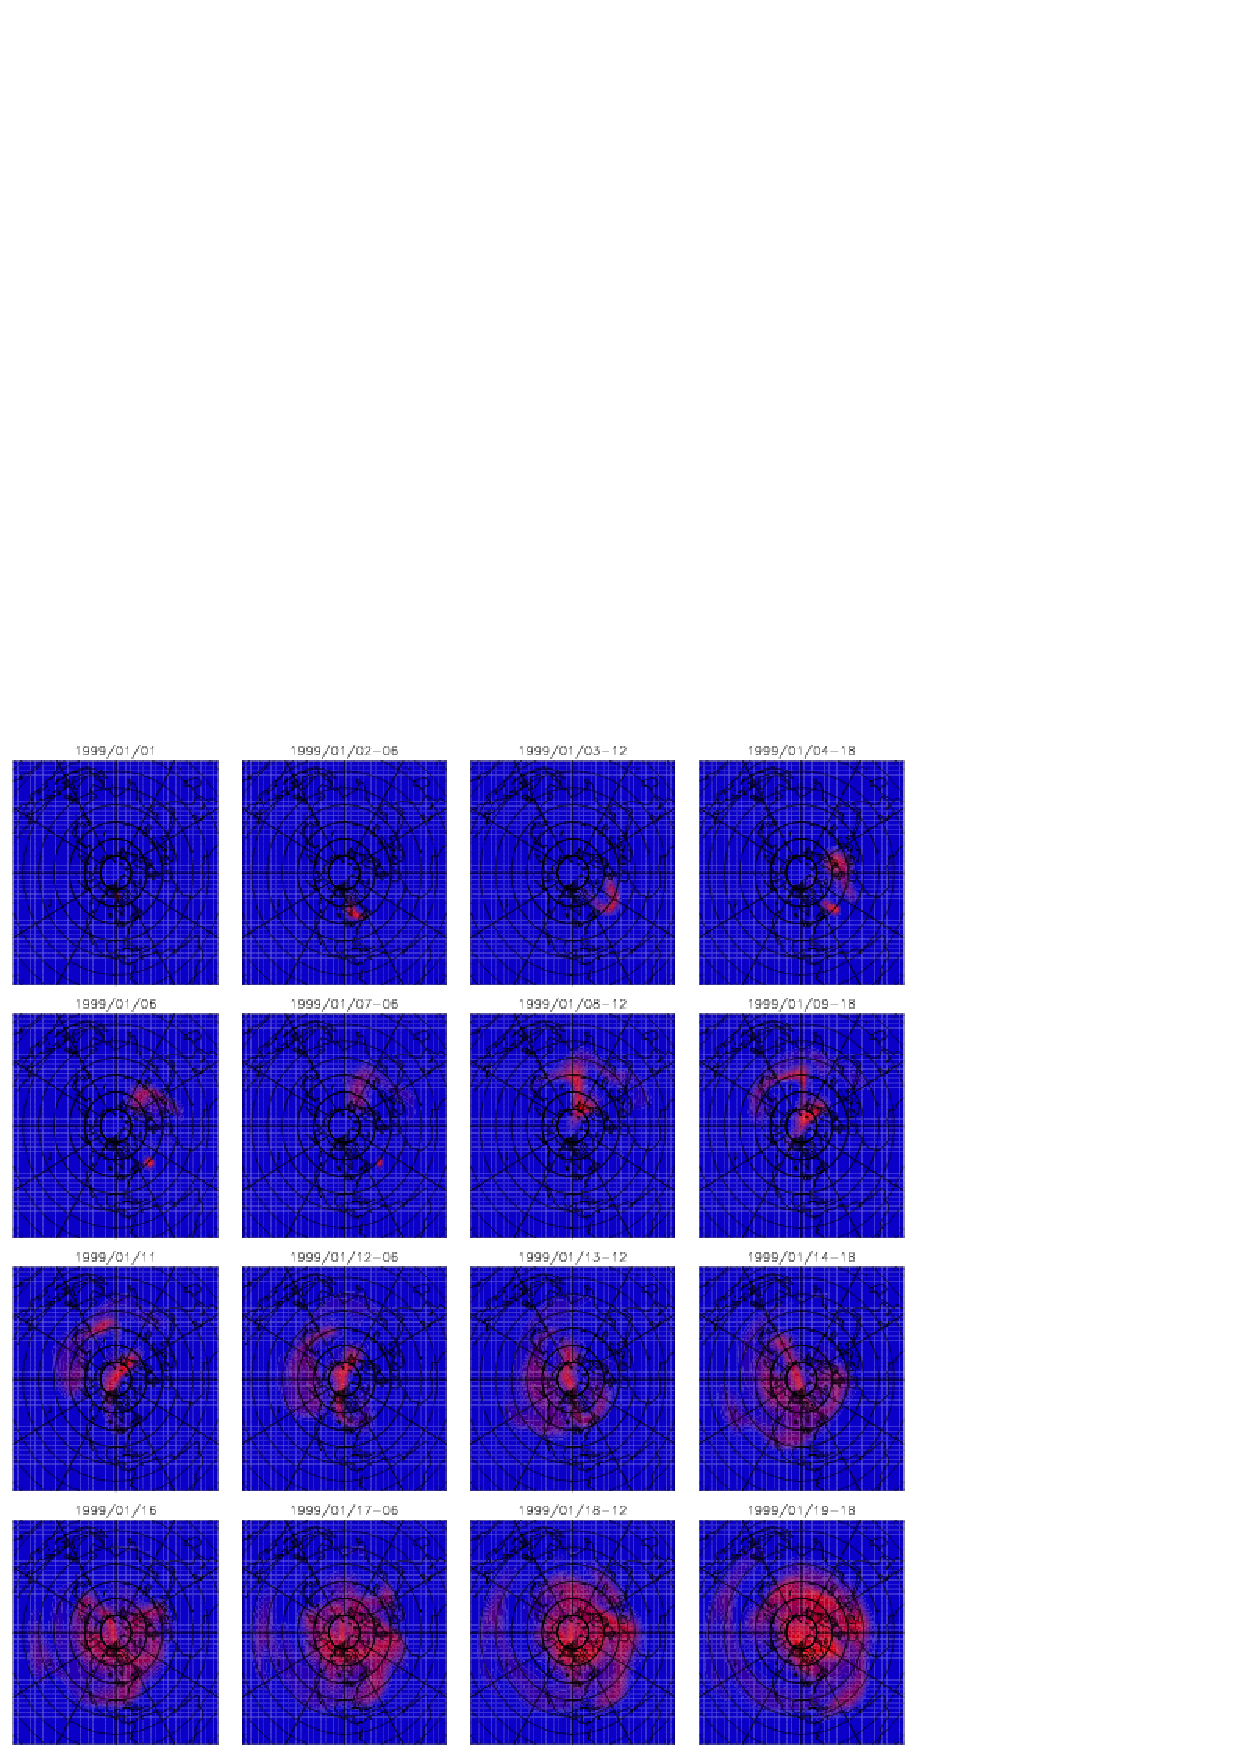
\includegraphics[width=0.5\textwidth]{tt_cover_graphic}
\end{center}

\pagestyle{myheadings}
\markright{Mills: Tracer Transport}

%\section*{Abstract}
\begin{abstract}
We review matrix methods as applied to tracer transport.
Because tracer transport is linear, matrix methods are an ideal
fit for the problem.  In particular,
solutions of linear, first-order systems of ordinary differential
equations (ODEs) are reviewed as well as 
special properties of these solutions.
Detailed derivations are included.
\end{abstract}

\subsection*{Keywords}
\textbf{tracer dynamics, Eulerian transport, numerical analysis, matrix methods, partial differential equations, ordinary differential equations, advection}

\tableofcontents

\section{Introduction}

\citet{Mills2012} introduces a method of dynamical tracer interpolation
in which the tracer dynamics are represented as a matrix and the largest
principal components correlated with a series of sparse measurements.
The method is called ``principal component proxy tracer analysis''.

Because such processes are linear, matrix methods represent a powerful and
general set of techniques to apply to problems in tracer advection and the
related issues of mixing and stretching.
This review summarizes some of these techniques as well as special properties
of the matrices as used to represent transport processes.  In particular, 
we review methods of solving systems of linear ordinary differential
equations (ODEs) of the form:
\begin{equation}
\frac{\mathrm d \vec r(t)}{\mathrm d t} = A(t) \cdot \vec r(t)
\end{equation}
where $A$ is the instantaneous dynamics, while $\vec r$ is either the tracer,
the stretching of an infinitessimal area in Lagrangian space or the tracer gradient at a single point
in Lagrangian space. 

The solution can be represented in the form:
\begin{equation}
\vec r(t)=R \cdot \vec r(t_0)
\end{equation}
The solution matrix, $R$, can be broken down in a number of useful ways
and may possess important properties depending upon those of $A$.  

It is hoped that this compilation
can help improve understanding of fluid transport and in particular 
improve both understanding and implementation of principal component
proxy and similar techniques.

\section{Fundamentals}

A trajectory is the motion in time of an infinitesimal packet of fluid
as it is carried along by the flow:
\begin{equation}
	\frac{\mathrm d \vec x}{\mathrm d t}=\vec v(\vec x,~t) \label{trajectory_equation}
\end{equation}
where $\vec x$ is position, $t$ is time and $\vec v$ is the flow field.
If we integrate this in time, starting at $t_0$ and ending at $t=t_0+\Delta t$, we get a
vector function, call it, $\Phi$:
\begin{equation}
	\vec x=\Phi(\vec x_0,~t_0,~\Delta t)
\label{traj_def}
\end{equation}
where $x_0=x(t_0)$ is the Lagrangian or starting coordinate.
Unlike in \citet{Ottino1989}, we specify the starting time explicitly instead 
of assuming that $t_0=0$.  This convention will become useful later on, e.g., 
when chaining functions:
\begin{equation}
\vec x=\Phi(\vec x_0,~\Delta t_1+\Delta t_2)=\Phi[\Phi(\vec x_0,~t_0,~\Delta t_1),~t_0 + \Delta t_1,~\Delta t_2]
\label{traj_fun_chaining}
\end{equation}

A flow tracer is a scalar field that follows the flow, typically a dissolved
trace substance, but could also comprise a suspension or in fact any property
of the fluid such as temperature or the velocity field itself.

The change in the total amount of tracer in a fixed volume, $\delta V$, is given
by the flux plus the source term:
\begin{equation}
	\frac{\partial}{\partial t}\int_{\delta V} \rho \mathrm d \vec x=-\oint_A \rho \vec v \cdot \hat n \mathrm d A
	+ \int_{\delta V} \sigma \mathrm d \vec x
	\label{volume_conservation_integral}
\end{equation}
where $\rho$ is the density of the tracer,
$A$ is the area enclosing $\delta V$ and $\sigma$ is the source term, which for the moment,
we will take to be zero but in later analysis will 
be needed both for the diffusion term and for explicit generation and loss terms.

From divergence theorem:
\begin{equation}
	\int_{\delta V} \frac{\partial \rho}{\partial t} \mathrm d \vec x=-\int_{\delta V} \nabla \cdot (\rho \vec v)\mathrm d \vec x 
\end{equation}
Removing the integrals and expanding the first term on the right side:
\begin{equation}
\frac{\partial \rho}{\partial t} =-\vec v \cdot \nabla \rho - \rho \nabla \cdot \vec v 
\label{mass_conservation_Eulerian}
\end{equation}
The first term is the advection term while the second term is the mass
conservation term and is governed by the 
expansion and contraction of the fluid.  In an incompressible fluid (that is,
$\nabla \cdot \vec v = 0$), this term will be zero.

To go from the {\it Lagrangian} to the {\it Eulerian formulation}, 
we use the following equation for the {\it total derivative}:
\begin{equation}
\frac{\mathrm d \rho}{\mathrm d t}
 = \frac{\partial \rho}{\partial t} + \vec v \cdot \nabla \rho
\end{equation}
Combining this with Equation (\ref{mass_conservation_Eulerian}):
\begin{equation}
\frac{\mathrm d \rho}{\mathrm d t} =  - \rho \nabla \cdot \vec v
\label{mass_conservation_Lagrangian}
\end{equation}
This is the Lagrangian equation for conservation of mass and governs the total density
of the fluid, that is, fluid density is itself a flow tracer.

Suppose we use a {\it mixing ratio} instead of density to track the
tracer:
\begin{equation}
	q = \frac {\rho}{\rho_t} \label{mixing_ratio}
\end{equation}
where $\rho_t$ is the total density of the fluid.  Differentiating this wrt
$t$ and then substituting Equation (\ref{mass_conservation_Lagrangian})
produces the following:
\begin{eqnarray}
\frac{\mathrm d q}{\mathrm d t} & = & \frac{1}{\rho_t} \frac{\mathrm d \rho}{\mathrm d t}
	- \frac{\rho}{\rho_t^2}\frac{\mathrm d \rho_t}{\mathrm d t}\\
& = & 0
\end{eqnarray}
or, in Eulerian form:
\begin{equation}
\frac{\partial q}{\partial t} = - \vec v \cdot \nabla q
\label{advection_eqn}
\end{equation}
This is the {\it advection equation}.

\section{Volume deformation}

\label{deformation_section}

Most of this analysis can be found in \citet{Pattanayak2001} and 
\citet{Mills2004}. 
%however we repeat it here since I seem to end up re-deriving
%it roughly every eight months.
The instantaneous rate of stretching of Lagrangian space is given by the
gradient, or Jacobi matrix, of the velocity, $\nabla \vec v$.
Suppose we perturb a trajectory by a minute amount, $\delta \vec x$.
The Tayler expansion of the time derivative is, to first order:
\begin{equation}
\frac{\mathrm d}{\mathrm d t} (\vec x + \delta \vec x) \approx
\vec v + \nabla \vec v \cdot \delta \vec x \label{taylor_expansion}
\end{equation}
or:
\begin{equation}
\frac{\mathrm d}{\mathrm d t}\delta \vec x \approx \nabla \vec v \cdot \delta \vec x
\label{evolution_error_vector}
\end{equation}
Whether we left multiply or right multiply depends on which convention we adopt
for the application of the gradient or nabla operator, $\nabla$, to a vector,
therefore we write it out component-by-component:
\begin{equation}
\nabla \vec v = \left [
\begin{array}{ccc}
\frac{\partial v_x}{\partial x} & \frac{\partial v_x}{\partial y} & \frac{\partial v_x}{\partial z} \\
\frac{\partial v_y}{\partial x} & \frac{\partial v_y}{\partial y} & \frac{\partial v_y}{\partial z} \\
\frac{\partial v_z}{\partial x} & \frac{\partial v_z}{\partial y} & \frac{\partial v_z}{\partial z}
\end{array} \right ]
\end{equation}
where $\vec x=[x_1,~x_2,~x_3]=[x,~y,~z]$.

We define $H(\vec x_0,~t_0,~\Delta t)$ as follows:
\begin{eqnarray}
\frac{\mathrm d H}{\mathrm d t} & = & \nabla \vec v \cdot H \\
\label{deformation_matrix}
H(\vec x_0,~t_0,~0) & = & I
\end{eqnarray}
where $I$ is the identity matrix.
This is known as the {\it tangent model} of a dynamical system and applied
to a trajectory is the total stretching of Lagrangian space.

We can relate $H$ to the integrated trajectory, $\Phi$, as follows:
\begin{eqnarray}
\frac{\mathrm d \Phi}{\mathrm d t} & = & v(\Phi, ~t) \\
%yes, the two operators do commute... duh...
\frac{\mathrm d}{\mathrm d t} 
\nabla_{\vec x_0} \Phi & = & \nabla \vec v \cdot \nabla_{\vec x_0} \Phi
\label{gradient_trajectory}
\end{eqnarray}
or,
\begin{equation}
\nabla_{\vec x_0} \Phi = H
\end{equation}
Note that:
\begin{equation}
	\delta \vec x = H \cdot \delta \vec x_0
	\label{initial_error_vector}
\end{equation}
where $\delta \vec x_0=\delta \vec x(t=t_0)$.

In conjunction with the equations for the evolution of error vectors, above,
we can derive a set of corresponding equations for the evolution of the tracer
gradient.  Taking the gradient of Equation (\ref{advection_eqn}):
\begin{equation}
\frac{\partial}{\partial t} \nabla q = -\nabla q \cdot \nabla \vec v -
		\vec v \cdot \nabla \nabla q
\end{equation}
Meanwhile, using the total derivative:
\begin{equation}
\frac{\mathrm d}{\mathrm d t} \nabla q = \vec v \cdot \nabla \nabla q \cdot + 
		\frac{\partial}{\partial t} \nabla q
\end{equation}
and combining the two:
\begin{equation}
\frac{\mathrm d}{\mathrm d t} \nabla q = -\nabla q \cdot \nabla \vec v
\label{evolution_tracer_gradient}
\end{equation}

In parallel with $H$, we define $H^\prime$:
\begin{eqnarray}
\frac{\mathrm d H^\prime}{\mathrm d t} & = & -H^\prime \cdot \nabla \vec v\\
\label{inverse_deformation_matrix}
H^\prime(\vec x_0,~t_0,~0) & = & I
\end{eqnarray}
It is easy to show that:
\begin{equation}
H^{-1}=H^\prime
\end{equation}
by taking the time derivative of $H^\prime \cdot H$:
\begin{eqnarray}
\frac{\mathrm d}{\mathrm d t} H^\prime \cdot H & = & 
		H^\prime \cdot \frac{\mathrm d H}{\mathrm d t} +
		\frac{\mathrm d H^\prime}{\mathrm d t} \cdot H\\
		& = & H^\prime \cdot \nabla \vec v \cdot H 
		- H^\prime \cdot \nabla \vec v \cdot H \\
		& = & 0
\end{eqnarray}
and that:
\begin{equation}
\nabla q = \nabla q_0 \cdot H^\prime
\end{equation}

Also, by defining $\Phi^{-1}(\vec x,~t,~\Delta t)$ as,
\begin{equation}
\Phi^{-1}[\Phi(\vec x_0,~t_0,~\Delta t),~t_0,~\Delta t]=\vec x_0
\end{equation}
we can show:
\begin{equation}
H^\prime=\nabla \Phi^{-1}
\end{equation}

\section{Transport map}

\label{map_section}

The dynamics of the tracer, $q$, can be summarized using a linear
{\it transport map}, $Q$:
\begin{equation}
	q(\vec x,~t)=\int_{V} Q(\vec x_0,~\vec x,~t_0,~\Delta t) q(\vec x_0,~t_0) \mathrm d \vec x_0
\label{tracer_map_continuous}
\end{equation}
where $V$ here represents the total volume.
In the absence of diffusion or source terms, this map can be calculated in
at least two ways, by a differential equation: 
\begin{eqnarray}
	\frac{\partial}{\partial t} Q & = & (\vec v \cdot \nabla) Q 
\label{tracer_map_continuous1}\\
Q(\vec x_0,~\vec x,~t_0,~0) & = & \delta(\vec x-\vec x_0) 
\label{tracer_map_continuous2}
\end{eqnarray}
where $\delta$ is the delta function, and using the trajectory function:
\begin{equation}
Q(\vec x_0,~\vec x,~t_0,~\Delta t) = \delta[\Phi(\vec x_0,~t_0,~\Delta t)-\vec x]
\label{tracer_map_continuous3}
\end{equation}
In the latter case, combination with (\ref{tracer_map_continuous}) produces the
Frobenius-Perron equation. \citep{Ott1993}

The transport map can be approximated by a matrix:
\begin{equation}
\vec q(t) = R \cdot \vec q(t_0)
\label{discrete_tracer_map0}
\end{equation}
where $\vec q$ is a discrete approximation of the tracer configuration:
$q_i = q(\vec x_i)$.  Tracer transport is fully linear and the time evolution
of $R$ is governed by the same mathematics as $H$ and $H^\prime$:
\begin{equation}
\frac{\mathrm d R}{\mathrm d t} = A \cdot R
\label{discrete_tracer_map}
\end{equation}
There are a number of ways to calculate $A$, the most obvious being from an 
Eulerian finite difference scheme, which, in one dimension, would look something
like this:
\begin{equation}
\frac{\mathrm d r_{ij}}{\mathrm d t} = \frac{v(x_j,~t)}{\Delta x_{j-1}+\Delta x_j} (r_{i,j+1} - r_{i,j-1})
\label{simple_finite_difference}
\end{equation}
or,
\begin{eqnarray}
a_{i-1,i} & = & - \frac{v(x_i,~t)}{\Delta x_{i-1}+\Delta x_i} \\
a_{i+1,i} & = & \frac{v(x_i,~t)}{\Delta x_{i-1}+\Delta x_i}
\end{eqnarray}
Neither representation shows the {\it boundary conditons}.  Typically, $A$
will be either band diagonal or, as in the case of a semi-Lagrangian
scheme, quite close.

For simplicity, we will analysize both this system and the pair of systems
discussed in the previous section using matrix algebra.  A more thorough
treatment would use abstract algebra and operator theory, especially for
the transport map.

\section{Matrix solution of systems of linear ODEs} 

\subsection{Analytic solution of the stationary case}

We wish to solve the system of linear ordinary differential equations (ODEs):
\begin{equation}
\frac{\mathrm d \vec r}{\mathrm d t}=A \cdot \vec r
\label{linear_ODE_system_vector_soln}
\end{equation}
Supposing $A$ has no time dependence, we perform an eigenvector 
decomposion:
\begin{equation}
  A = T \cdot \Lambda \cdot T^{-1}
  \label{eigenvalue_expansion}
\end{equation}
where $T$ is a matrix of right eigenvectors, and $\Lambda$ is a diagonal matrix
of eigenvalues, $\lambda_{ii}=\lambda_i \ge \lambda_{i-1}$.  
The left eigenvectors are contained in $T^{-1}$.
Thus,
\begin{equation}
  \frac{\mathrm d}{\mathrm d t} T^{-1} \cdot \vec r=\Lambda \cdot T^{-1} \cdot  \vec r
\end{equation}
By performing the linear coordinate transformation,
\begin{equation}
  \vec r^\prime=T^{-1} \cdot \vec r
\end{equation}
the equation is easily solved:
\begin{equation}
r^\prime_i = e^{\lambda_i \Delta t} r^\prime_i(t=t_0)
\end{equation}
or, in the un-transformed system:
\begin{eqnarray}
  \vec r & = & \left [T \cdot \exp(\Delta t \Lambda) \cdot T^{-1} \right ] \cdot \vec r_0 
\label{solution_no_time_dependence} \\
& \equiv & \exp(\Delta t A)\cdot \vec r_0
\end{eqnarray}
where $\vec r_0=\vec r(t_0)$.

\subsection{Solving the time-dependent case}

The stationary case is interesting, but what can it tell us about the 
more general case in which $A$, which we'll call the {\it evolution matrix},
is time-dependent?
We can generalize the problem further as in (\ref{deformation_matrix}) and
(\ref{inverse_deformation_matrix}) so that a matrix, $R$, 
is used in place of the vector, $\vec r$:
\begin{equation}
\frac{\mathrm d R}{\mathrm d t}=A(t) \cdot R
\label{linear_ODE_system_matrix_soln}
\end{equation}
One of the most important properties of the solution is that it
is decomposable as follows:
\begin{equation}
	R(t_0,~t_n-t_0) = R(t_n,\,\Delta t_n) \cdot R(t_{n-1},\,\Delta t_{n-1}) \cdot R(t_{n-2},\,\Delta t_{n-2}) \cdot \, ...~~ 
	\cdot R(t_0,\,\Delta t_0)
\label{matrix_soln_decomposition}
\end{equation}
where,
\begin{equation}
t_n=t_0+\sum_{i=0}^n \Delta t_i
\end{equation}
and we have used the convention, begun
in Equation (\ref{traj_def}) of making $R$ a function both of the
initial time and of the subsequent time interval.  
It follows that $R(t, 0)=I$.

Going back to Equation (\ref{linear_ODE_system_vector_soln}), we can
see that the vector solution is given by a product of the initial vector with
the matrix solution:
\begin{equation}
\vec r(t_0+\Delta t)=R(t_0, \Delta t) \cdot \vec r(t_0)
\end{equation}

It stands to reason that each element in the decomposition in (\ref{matrix_soln_decomposition})
may be approximated by the stationary solution in the limit as the time step
approaches zero:
\begin{equation}
R(t, ~ \Delta t \rightarrow 0) = \exp \left [ A(t) \Delta t \right ]
\end{equation}

\subsection{Negative and left-multiplied cases}

Consider the case in which the order of the factors on the R.H.S of Equation 
(\ref{linear_ODE_system_vector_soln}) are reversed (left-multiply vs. right-multiply):
\begin{equation}
\frac{\mathrm d \vec r}{\mathrm d t} = \vec r \cdot A
\end{equation}
This case is particularly important, since Equation (\ref{evolution_error_vector})
when rearranged in this way becomes the vorticity equation \citep{Acheson1990}.

We start with the analytic solution of the stationary case:
\begin{eqnarray}
  A & = & T \cdot \Lambda \cdot T^{-1} \\
  \frac{\mathrm d \vec r}{\mathrm d t} & = & \vec r \cdot T \cdot \Lambda \cdot T^{-1} \\
  \frac{\mathrm d}{\mathrm d t} (\vec r \cdot T) & = & (\vec r \cdot T) \cdot \Lambda \\
  \vec r \cdot T & = & \vec r_0 \cdot T \cdot \exp (\Lambda t) \\
	\vec r & = & \vec r_0 \cdot T \cdot \exp (\Lambda t) \cdot T^{-1}
\end{eqnarray}
In other words, the solution is the same, but the initial conditions are
left-multiplied instead of right multiplied, or equivalently, the whole thing 
could be transposed.

In the time-dependent case each element of the solution is in reverse order,
not just the initial conditions:
\begin{equation}
	\vec r(t_n) = \vec r_0 \cdot R^*(t_0,\Delta t_0) \cdot R^*(t_1, \Delta t_1) \cdot \cdot R^*(t_2, \Delta t_2) ~ ... 
~ \cdot R^*(t_n,\Delta t_n)
\end{equation}
where $R^*$ is a solution to the equation:
\begin{eqnarray}
\frac{\mathrm d}{\mathrm d t}R^*(t_0,~t) & = & R^*(t_0, ~t) \cdot A(t) \\
R^*(t_0, ~ 0) & = & I
\end{eqnarray}
and,
\begin{equation}
R^*(t,~\Delta t \rightarrow 0) = R(t,~ \Delta t ) 
 = \exp \left [ A(t) \Delta t \right ]
\end{equation}

For the case of a negative R.H.S.:
\begin{equation}
\frac{\mathrm d \vec r}{\mathrm d t} = - A \cdot \vec r
\end{equation}
it is easy to show that the stationary solution is simply inverted:
\begin{eqnarray}
  \vec r & = & T \cdot \exp (-\Lambda t) \cdot T^{-1} \cdot \vec r \\
	& = & T \cdot \left [ \exp (\Lambda t) \right ]^{-1} \cdot T^{-1} \cdot \vec r \\
 & = & \left [T \cdot \exp (\Lambda t) \cdot T^{-1} \right]^{-1} \cdot \vec r 
\end{eqnarray}
while for the time-dependent case, we have:
\begin{equation}
	\vec r \approx R^{-1}(t_n,\Delta t_n) \cdot R^{-1}(t_{n-1},\Delta t_{n-1}) \cdot R^{-1}(t_{n-2}, \Delta t_{n-2}) \cdot ~ ... 
~ \cdot R^{-1}(t_0,\Delta t_0) \cdot \vec r_0
\end{equation}
assuming that each $\Delta t_i$ is small enough that $R$ approximates the 
stationary case.
This provides an alternative derivation for the solution of the negative,
transposed (left-multiplied) case which we saw already in (\ref{evolution_tracer_gradient}):
\begin{equation}
\frac{\mathrm d R}{\mathrm d t} = -\vec r \cdot A
\end{equation}
which is given by:
\begin{eqnarray}
\vec r(t_n) & \approx & \vec r_0 \cdot R^{-1}(t_0,\Delta t_0) \cdot R^{-1}(t_1, \Delta t_1) \cdot ~ ... 
~ \nonumber \\
& & ~~~~~~~...~\cdot R^{-1}(t_{n-1},\Delta t_{n-1}) \cdot R^{-1}(t_n,\Delta t_n) \\
& = & \vec r_0 \cdot R^{-1}(t_0, t_n-t_0)
\end{eqnarray}
Where $R$ is the solution to Equation (\ref{linear_ODE_system_matrix_soln}).

\section{SVD and the Lyapunov spectrum}

The singular value decomposition of a matrix is given as:
\begin{equation}
R=U\cdot S\cdot V^T
\label{SVD_def}
\end{equation}
where $R$ is an $[m \times n]$ matrix, $U$ is an $[m \times n]$ ortho-normal
matrix, $S$ is an $[n \times n]$ diagonal matrix of {\it singular values}
($s_{ii}=s_i>s_{i+1}$) and $V$ is an $[n \times n]$ ortho-normal matrix.

$U$ and $V^T$ are also termed the left and right {\it singular vectors}, 
respectively and are normally calculated through eigenvalue analysis:
\begin{eqnarray}
	R\cdot R^T \cdot U & = & U \cdot S^2 \label{left_SV_eigenproblem}\\
	R^T \cdot R \cdot V & = & V \cdot S^2 \label{right_SV_eigenproblem}
\end{eqnarray}
Typically, only one of $U$ or $V$ is calculated and then the other by projection
onto $R$.  Which one is calculated first is best determined by whether $m$
is greater than or less than $n$.  Equation (\ref{SVD_def}) assumes that 
$m>n$. 
For all the problems discussed in this review, $m=n$.

Because both $R^T \cdot R$ and $R \cdot R^T$ are symmetric
the singular values,
$\lbrace s_i \rbrace$, are always real.
Moreover, the eigenvectors in $U$ and $V$ form an orthogonal set spanning the
space and by convention are normalized so that,
$U^T \cdot U = V^T \cdot V = I$.

Assuming that $R$ is an integrated tangent model as in 
(\ref{deformation_matrix}), (\ref{inverse_deformation_matrix})
and (\ref{discrete_tracer_map}), 
the Lyapunov exponents are defined as the time averages of the logarithms
of the singular values in the limit as time goes to infinity:
\begin{equation}
h_i=\lim_{\Delta t \rightarrow \infty} \frac{1}{\Delta t} \log s_i
\label{Lyap_def}
\end{equation}

If there is any significant difference between the largest and next largest
Lyapunov exponents, the largest singular value will come to dominate the matrix
as it evolves forward in time.  Thus:
\begin{equation}
r_i(t \rightarrow \infty) = u_{i1} s_1 \sum_j v_{j1} r_j(t_0)
\end{equation}
and:
\begin{equation}
|\vec r(t \rightarrow \infty)| = |\vec r_0| e^{h_1 \Delta t}
\label{large_Lyap}
\end{equation}
The Lyapunov exponent is often somewhat incorrectly defined as
(\ref{large_Lyap}) above.

\section{Special properties}

Since each element in (\ref{matrix_soln_decomposition}) approaches the
non-time-dependent solution given by the first factor of 
(\ref{solution_no_time_dependence}) in the limit as $\Delta t_i\rightarrow 0$, 
we can use the properties of the non-time-dependent solution to
reason about those of the time-dependent one.
In many cases of the problems discussed in Section \ref{deformation_section}
and Section \ref{map_section}, the evolution matrix, $A$, will have
special properties that will affect the solution.

\subsection{Volume conservation}

In the solution of (\ref{deformation_matrix}) for instance, 
$A=\nabla \vec v$, while the velocity field, $\vec v$, is frequently non-divergent,
that is $\nabla \cdot \vec v=0$ or $\mathrm{Tr}(A)=0$.
It can be shown that 
if the trace of a matrix is zero, then the eigenvalues sum to zero.
We provide a brief outline of the proof.

We begin by writing the characteristic polynomial as follows:
\begin{equation}
  \lambda^n + k_1 \lambda^{n-1} + k_2 \lambda^{n-2} + ~... ~
  + k_{n-2} \lambda + k_{n-1} \lambda + k_n = 0
\end{equation}
The first coefficient, $k_1$, is always given as:
\begin{equation}
	k_1 = a_{11} + a_{22} + a_{33} + ~ ... ~ = \mathrm{Tr}(A)
\end{equation}
We can rewrite the characteristic polynomial
in terms of the roots:
\begin{eqnarray}
	& (\lambda - \lambda_1)(\lambda - \lambda_2)(\lambda-\lambda_3) ~ ... \\
	= & \lambda^n + (\lambda_1 + \lambda_2 + \lambda_3 + ~ ...) \lambda^{n-1} + ...
\end{eqnarray}
Thus:
\begin{equation}
	k_1 = \mathrm{Tr}(A) = \sum_i \lambda_i = 0
\end{equation}

The determinant of the stationary solution matrix,
$R=T\cdot\exp(\Delta t\Lambda)\cdot T^{-1}$, in (\ref{solution_no_time_dependence}) is:
\begin{eqnarray}
	|R| & = & |T||\exp(\Delta t\Lambda)||T^{-1}| \\
	    & = & |T| \left [ \prod_i \exp(\Delta t \lambda_i) \right ] \frac{1}{|T|} \\
& = & \exp\left(\Delta t \sum_i \lambda_i\right) \\
& = & 1
\end{eqnarray}
In other words, the solution, in this case, is {\it volume-conserving}:
volumes in the space, e.g. as calculated by the determinant of a set of 
solution vectors
spanning the space, are conserved.  
This is known as Liouville Theorem \citep{Thornton2003}.

The result generalizes to the time-dependent case since the solution can
always be decomposed as an infinite product of infinitessimally small 
stationary integrations.
Like the eigenvalues, the Lyapunov exponents will also sum to zero:
\begin{eqnarray}
|R| =	|U||S||V^T| & = & 1 \\
	\prod_i s_i & = & 1 \\
	\prod_i \exp(\Delta t h_i) & = & 1 \\
	\sum_i h_i & = & 0
\end{eqnarray}


\subsection{Mass and length conservation}

Suppose $R$ has the property that it preserves lengths when applied to
a vector:
\begin{equation}
|R\cdot \vec q| = |\vec q|
\label{length_preservation}
\end{equation}
thus the rate of change of the vector will always be perpendicular:
\begin{eqnarray}
\frac{\mathrm d}{\mathrm d t}|\vec q| & = & 
	\nabla |\vec q| \cdot \frac{\mathrm d \vec q}{\mathrm d t} \\
	&=& \frac{\vec q}{|\vec q|} \cdot A \cdot \vec q \\
	&=& 0 \\
	\vec q \cdot A \cdot \vec q & = & 0 
\end{eqnarray}
$A$ is what we shall call an ``orthogonality transform''.
By separating the diagonal and off-diagonal components in the last expression,
\begin{equation}
\sum_i \sum_j a_{ij} q_i q_j = \sum_{i=1}^n a_{ii}q_i^2 + \sum_{i=1}^n \sum_{j=i+1}^n (a_{ij} q_i q_j + a_{ji} q_i q_j) = 0
\end{equation}
we can show that it has the following
properties:
\begin{eqnarray}
a_{ii} & = & 0 \\
a_{ij}+a_{ji} & = & 0
\end{eqnarray}

Meanwhile, $R$ is a rotation.  All the singular values of $R$ will be $1$:
\begin{equation}
	\vec q \cdot R^T \cdot R \cdot \vec q = \vec q \cdot \vec q \label{length_conservation}
\end{equation}
This implies:
\begin{eqnarray}
R^T \cdot R \cdot \vec v & = & s^2 \vec v \nonumber \\
	s & = & 1 \label{ortho_eigen}
\end{eqnarray}
or perhaps more simply:
\begin{equation}
	R^T \cdot R \cdot \vec v = I \vec v = s^2 \vec v \\
\end{equation}
Because it is a rotation, it will be orthonormal with a determinant of 1.

The tracer mapping, $Q$, as defined in 
(\ref{tracer_map_continuous1}) and (\ref{tracer_map_continuous2}),
that is, without diffusion, will fulfill these properties.  Discrete mappings
can only approximate them and by necessity always include some diffusion.

A more important property of tracer advection is that the total substance
remains constant, thus:
\begin{eqnarray}
\sum_i q_i & = & const. \\
\frac{\mathrm d}{\mathrm d t}\sum_i q_i & = & 0
\end{eqnarray}
This will be true even if $q$ is measured as a mixing ratio, provided that
the flow is non-divergent.  
It also assumes, of course, an equal-volume grid.
Most flows in real fluids are approximately 
non-divergent, especially when considered over long time scales.
Continuing the derivation:
\begin{eqnarray}
\sum_i \sum_j r_{ij} q_j & = & \sum_j q_j \\
\sum_j q_j \left ( \sum_i r_{ij} - 1 \right ) & = & 0
\end{eqnarray}
and:
\begin{eqnarray}
\sum_i \frac{\mathrm d q_i}{\mathrm d t} & = & 0 \\
\sum_i \sum_j a_{ij} q_j & = & 0 \\
\sum_j q_j \sum_i a_{ij} & = & 0 
\end{eqnarray}
Therefore:
\begin{eqnarray}
\sum_i r_{ij} & = & 1 
\label{column_sums_to_one}\\
\sum_i a_{ij} & = & 0
\label{column_sums_to_zero}\\
\end{eqnarray}
%[Problem: show that the second property implies the first using an eigenvalue
%solution for an A with no time dependence.]

For grids that aren't equal-volume, we apply the following transformations:
\begin{equation}
  \tilde q_i = w_i q_i
\end{equation}
where $w_i$ is a weight accounting for the relative differences 
in volume at the $i$th grid point.
The relevant matrices will also need to be transformed:
\begin{eqnarray}
  \tilde r_{ij} & = & \frac{w_i}{w_j} r_{ij} \\
  \tilde a_{ij} & = & \frac{w_i}{w_j} a_{ij}
\end{eqnarray}
The same constraints in 
(\ref{column_sums_to_one}) and (\ref{column_sums_to_zero}) 
now apply to the transformed matrices, $\tilde R=\lbrace \tilde r_{ij} \rbrace$
and $\tilde A=\lbrace \tilde a_{ij} \rbrace$.
If the weights are given time dependence, a similar method can be
applied to account for local changes in density in non-divergent flows.

As pointed out already, a discrete tracer mapping will always require some 
amount of diffusion.  This means that the tracer configuration will 
tend towards a uniform distribution over time, 
that is, it will ``flatten out.''  We can
show that, given the above constraint, a tracer field with all the same values
 has the smallest magnitude.  Suppose there are only two elements in the 
tracer vector, $\vec q=\lbrace q,~q \rbrace$.  The magnitude of the vector is:
\begin{equation}
|\vec q|=\sqrt{q^2+q^2}=\sqrt{2} q
\end{equation}
Now we introduce a separation between the elements, $2\Delta q$, that 
nonetheless keeps the sum of the elements constant:
\begin{eqnarray}
|q+\Delta q,~q-\Delta q| & = & \sqrt{(q+\Delta q)^2+(q-\Delta q)^2} \\
& = & \sqrt{2}\sqrt{q^2+(\Delta q)^2} \ge \sqrt{2} q
\end{eqnarray}
This will generalize to higher-dimensional vectors.  In general, we can
say that:
\begin{equation}
\vec q \cdot R^T \cdot R \cdot \vec q \le \vec q \cdot \vec q
\label{tracer_map_inequality}
\end{equation}
Implying that for the eigenvalue problem,
\begin{eqnarray}
R^T \cdot R \cdot \vec v & = & s^2 \vec v \nonumber\\
s^2 & \le & 1 \label{SV_inequality}
\end{eqnarray}
This further shows that the Lyapunov exponents are all
either zero or negative with the largest equal to 0.  This has been shown
numerically in \citet{Mills2012}.
Note however that this does not constitute a proof; the actual proof is more 
involved.

To prove (\ref{SV_inequality}) from (\ref{tracer_map_inequality}), we first
expand $\vec q$ in terms of the right singular values, 
$\lbrace \vec v_i \rbrace$:
\begin{equation}
	\vec q = \sum_i c_i \vec v_i
\end{equation}
where $\lbrace c_i \rbrace$ are a set of coefficients.
Substituting this into the left-hand-side of (\ref{tracer_map_inequality}):
\begin{eqnarray}
	\vec q \cdot R^T \cdot R \cdot \vec q & = & \left ( \sum_i c_i \vec v_i \right ) \cdot \left (\sum_i c_i s_i^2 \vec v_i \right ) \\
   & = & \sum_i \sum_j c_i c_j s_i^2 \vec v_i \cdot \vec v_j \\
   & = & \sum_i \sum_j c_i c_j s_i^2 \delta_{ij} \\
	  & = & \sum_i c_i^2 s_i^2
\end{eqnarray}
where $\delta$ is the Kronecker delta.
Similarly, we can show that:
\begin{equation}
	\vec q \cdot \vec q = \sum_i c_i^2
\end{equation}
If we assume that $s_i \le 1$ for every $i$, then:
\begin{equation}
	\sum_i c_i^2 s_i^2 \le \sum_i c_i^2 
	\label{diffusive_inequality_in_terms_of_SVs}
\end{equation}
since each term on the left side is less-than-or-equal-to the
corresponding term on the right side. 
Note that in order for the inequality in 
(\ref{diffusive_inequality_in_terms_of_SVs}) to be broken, at least one
singular value must be greater-than one.
Therefore (\ref{tracer_map_inequality}) is true for every $\vec q$
if-and-only-if (\ref{SV_inequality}) is true for every $s$.
In the language of set theory and first-order logic:
\begin{equation}
	\forall \vec q \in \Re^n ~ (\vec q \cdot R^T \cdot R \cdot \vec q \le \vec q \cdot \vec q) \iff \forall s \in \Re | ~R^T \cdot R \cdot \vec v = s^2 \vec v ~ (s \le 1)
\end{equation}
A similar argument will prove (\ref{length_conservation})
iff (\ref{ortho_eigen}).

\section{Volume deformation versus the transport map}

Since the volume deformation matrices,
$H$ and $H^\prime$, and the transport map, $Q$, are all derived from the
transport equations, and their time evolution has the same mathematical form,
we would expect them to be closely related. 
The $H$ matrices describe the local deformation of Lagrangian space 
while $Q$ describes the global deformation.
Since $\delta \left [\Phi(\vec x_0) - \vec x \right ]=\delta \left [\vec x_0 - \Phi^{-1}(\vec x) \right ]$,
we can derive (\ref{inverse_deformation_matrix}) from
(\ref{tracer_map_continuous}) and (\ref{tracer_map_continuous3}) by taking 
the gradient of $q$:
\begin{eqnarray}
	\nabla_{\vec x} q & = & - \int_V \vec \delta^\prime \left [\vec x_0 - \Phi^{-1}(\vec x) \right ] q_0 (\vec x_0) 
	\mathrm d \vec x_0 \cdot \nabla_{\vec x} \Phi^{-1} \\
	& = & - \nabla_{\vec x_0} q_0 \cdot H^\prime
\end{eqnarray}
where $\vec \delta^\prime$ is the generalized vector derivative of the 
Dirac delta function.

Once we admit diffusion, the final tracer gradient is no longer locally 
dependent on the gradient at the starting point, but rather depends on the
whole initial tracer configuration:
\begin{equation}
	\nabla_{\vec x} q = \int_V \nabla_{\vec x} Q(\vec x_0, \vec x) q_0 (\vec x_0) \mathrm d \vec x_0
\end{equation}

As with $\Phi$ and $\Phi^\prime$, 
there will exist an inverse transport map, $Q^{-1}$, from which we can derive
$H$. In the absence of diffusion, the mathematics will be identical whether
we move forward or backward in time.
That is, for every $q_0$:
\begin{equation}
	\int_V Q^{-1}(\vec x, \vec x_0, t_0+\Delta t, \Delta t) 
	\int_V Q(\vec x_0^\prime, \vec x, t_0, \Delta t) 
	q_0(\vec x_0^\prime, t_0) 
	\mathrm d \vec x_0^\prime \mathrm d \vec x = q_0(\vec x_0, t_0)
\end{equation}
or:
\begin{eqnarray}
	& & \int_V  Q^{-1}(\vec x^\prime, \vec x_1, t_0+\Delta t, \Delta t)
	Q(\vec x_2, \vec x^\prime, t_0, \Delta t) \mathrm d \vec x^\prime \\
	& & = \int_V  Q^{-1}(\vec x^\prime, \vec x_1, t_0+\Delta t, \Delta t)
	Q(\vec x_2, \vec x^\prime, t_0, \Delta t) \mathrm d \vec x^\prime \\ 
	& & = \delta(\vec x_1 - \vec x_2)
\end{eqnarray}
For the non-diffusive case, $Q$ is a rotation and therefore orthogonal.
We construct the inverse by simply reversing the roles of the variables:
$Q^{-1}(\vec x, \vec x_0) = Q(\vec x_0, \vec x)$, 
the equivalent of the matrix transpose in the discrete case.

Of particular interest is what happens to these maps in the limit as time
goes to infinity, $\Delta t \rightarrow \infty$.
By SVD:
\begin{equation}
	\lim_{\Delta \rightarrow \infty} H^\prime = 
	s_{h^\prime1} \vec h_f^\prime \otimes \vec h_0^\prime
\end{equation}
where $\otimes$ is the outer product and $s_{h^\prime1}$ is the largest 
singular value. The tracer gradient becomes:
\begin{equation}
	\nabla_{\vec x} q = s_{h^\prime1} \vec h_f^\prime
	\nabla_{\vec x_0} q_0 \cdot \vec h_0^\prime
\end{equation}

Once we generalize SVD to continuous distributions, a similar thing will
be seen to happen with the transport map:
\begin{equation}
	\lim_{\Delta \rightarrow \infty} Q(\vec x_0, \vec x) =
	Q_f (\vec x) Q_0 (\vec x_0)
	\label{transport_map_separable}
\end{equation}
In other words, it has become separable and:
\begin{equation}
	\nabla_{\vec x} q = \nabla_{\vec x} Q_f \int_V Q_0 (\vec x_0) q_0 (\vec x_0) \mathrm d \vec x_0
\end{equation}
Note that no singular value has been included since we saw from
(\ref{SV_inequality}) that it should be close to unity.

In other words:
\begin{equation}
	\vec h_f^\prime \approx \frac{k}{s_{h^\prime1}} \nabla_{\vec x} Q_f
\end{equation}
where
\begin{equation}
	k \approx \frac{\int_V Q_0 (\vec x^\prime) q(\vec x^\prime) \mathrm d \vec x^\prime}
	{\nabla_{\vec x_0} q_0 \cdot \vec h_0^\prime}
\end{equation}
is a constant of proportionality.
Because (\ref{transport_map_separable}) is only true when diffusion is present,
the relationships will only be approximate.

\section{Practical considerations}

\label{practical_considerations}

The traditional method of testing Eulerian tracer simulations for stability
is von Neumann analysis.
Equation (\ref{simple_finite_difference}) provides a simple, finite
difference method for
calculating the evolution matrix, $A$, for an Eulerian tracer simulation.
Assuming we've obeyed the Courant-Friedrichs-Lewy (CFL) criterion for choosing
the time-step (which itself is derived from von Neumann analysis), von Neumann
analysis shows this method to be unconditionally stable.

In fact the method is quite naive and if applied to any real fluid flow would 
quickly overflow.
This is because shear flows and mixing cause the tracer gradient to grow without bound.
To fix this, some amount of diffusion must be added.  Here is the 
{\it advection-diffusion} equation:
\begin{equation}
\frac{\partial q}{\partial t} = - \vec v \cdot \nabla q + \nabla \cdot D \cdot \nabla q
\label{advection_diffusion}
\end{equation}
where $D$ is the diffusivity tensor.
Here is its translation, in one dimension, to a second-order, centred,
finite-difference equation with uniform spatial grids:
\begin{eqnarray}
\frac{\partial q_i}{\partial t} & = & \frac{v(q_{i+1} - q_{i-1})}{2 \Delta x} +
	\frac{d (q_{i-1} + q_{i+1} - 2 q_i)}{\Delta x^2} \\
& = & \left (- \frac{v}{2 \Delta x} + \frac{d}{\Delta x^2} \right ) q_{i-1} -
	\frac{2 d}{\Delta x^2} q_i + 
	\left (\frac{v}{2 \Delta x} + \frac{d}{\Delta x^2} \right ) q_{i+1} \label{finite_difference_diffusion}
\end{eqnarray}
where $d$ is a scalar diffusion coefficient.
Expressed as elements of a matrix:
\begin{eqnarray}
a_{i,i-1} & = & \left (- \frac{v}{2 \Delta x} + \frac{d}{\Delta x^2} \right ) \\
	a_{i,i} & = & -\frac{2 d}{\Delta x^2} \\
a_{i,i+1} & = & \left (\frac{v}{2 \Delta x} + \frac{d}{\Delta x^2} \right )
\end{eqnarray}
In order to prevent the simulation from overflowing, $d$ will have to be tuned.
Generalization to two or more dimensions is straightforward.
Since the simulation is discrete, the actual order of points in the
vector or matrix is arbitrary.

Semi-Lagrangian methods perform a back-trajectory from each of the Eulerian
points in the simulation, then interpolate the new value.  Rather than
directly integrating the tracer values, 
the interpolation coefficients are stored immediately
in the a transport matrix, $R(t_i,~\Delta t_i)$, skipping the integration
step.
Each Eulerian time-step produces one element in the decomposition of the
larger transport matrix $R(t_0,~t_n-t_0)$.

Semi-Lagrangian methods are unconditionally stable and not subject to the
CFL criterion.
Both the final transport map, and each member of its decomposition normally have
the following properties:
\begin{itemize}
\item every element is between 0 and 1:
\begin{equation}
0 \le r_{ij} \le 1
\label{element_on_unit_interval}
\end{equation}
\item rows sum to 1:
\begin{equation}
\sum_j r_{ij} = 1
\label{rowssumtoone}
\end{equation}
\end{itemize}
The first condition holds for linear interpolation methods which will have
a maximum of $2^N$ non-zero elements per row, 
where $N$ is the number of dimensions. 
Some kernel-smoothing methods include negative coefficients.

In addition, we can approximate the evolution matrix to second order:
\begin{equation}
A(t_i+\Delta t/2) \approx \frac{1}{\Delta t} \left [R(t_i,~\Delta t) - I \right ]
\end{equation}

\subsection{Criteria for stability}

If the transport map, $R$, satisfies both Equation (\ref{column_sums_to_one})
and the inequality in (\ref{element_on_unit_interval}) then it is mathematically
equivalent to a conditional probability.
In addition, if we normalize the tracer such that $\sum_i q_i=1$
then it too is equivalent to a probability.

By translating Equation (\ref{length_preservation}) into an inequality, 
we arrive at a pair of criteria for the evolution matrix:
\begin{eqnarray}
a_{ii} & \le & 0 \\
a_{ij}+a_{ji} & \le & 0
\end{eqnarray}
in agreement with our definition of a strictly diffusive transport map in
(\ref{tracer_map_inequality}). 


\section{Adding sources and sinks}

We wish to add a source term, $\vec \sigma$, to the matrix tracer model
described in the previous sections:
\begin{equation}
\frac{\mathrm d \vec q}{\mathrm d t} = A(t) \cdot \vec q + \vec \sigma(t)
\end{equation}
Integrating to a discrete, first order approximation:
\begin{eqnarray}
  \vec q(t_n) 
  & \approx & \Delta t_{n-1} \sigma(t_{n-1}) + \nonumber \\
  & & R(t_{n-1}, ~ \Delta t_{n-1}) \cdot [(\Delta t_{n-2} \vec \sigma(t_{n-2}) + \nonumber \\
  & & R(t_{n-2}, ~ \Delta t_{n-2}) \cdot [\Delta t_{n-3} \vec \sigma(t_{n-3}) + \nonumber \\
  & & ~... + \nonumber \\
  & & R(t_2, ~ \Delta t_2) \cdot [\Delta t_1 \vec \sigma(t_1) + \nonumber \\
  & & R(t_1, ~ \Delta t_1) \cdot [\Delta t_0 \vec \sigma(t_0) + \nonumber \\
  & & R(t_0, ~ \Delta t_0) \cdot q(t_0) ]]...]]
\end{eqnarray}
and multiplying through:
\begin{eqnarray}
\vec q(t_n) 
  & \approx & R(t_0, ~ t_n-t_0) \cdot \vec q(t_0) + \nonumber \\
  & & \Delta t_0 R(t_1, ~ t_n-t_1) \cdot \vec \sigma(t_0) + \nonumber \\
  & & \Delta t_1 R(t_2, ~ t_n-t_2) \cdot \sigma(t_1) + \nonumber \\
  & & ~...~+ \nonumber \\ 
  & & \Delta t_{n-3} R(t_{n-2}, ~ t_n-t_{n-2}) \cdot \vec\sigma(t_{n-3}) + \nonumber \\
  & & \Delta t_{n-2} R(t_{n-1}, ~ \Delta t_{n-1}) \cdot \vec \sigma(t_{n-2}) + \nonumber \\
  & & \Delta t_{n-1} \sigma(t_{n-1}) \\
  & = & R(t_0,~t_n-t_0) \cdot \vec q(t_0) + 
  \sum_{i=1}^{n} \Delta t_{i-1} R(t_i,~t_n-t_i) \cdot \vec \sigma(t_{i-1})
\end{eqnarray}

\subsection{Diffusion}

Unlike external sources and sinks, we can add diffusion to the model without
fundamentally changing it or its linearity. Consider the diffusion equation
in one dimension:
\begin{equation}
  \frac{\partial q}{\partial t}=d \frac{\partial^2 q}{\partial x^2}
\end{equation}
where $d$ is the diffusion coefficient.
Solving by separation of variables:
\begin{equation}
  q=q_0 e^{-d \omega^2 t} e^{i \omega x}
  \label{diffusion_solution}
\end{equation}
where $\omega$ is the angular frequency of a stationary wave
and $q_0$ is its initial amplitude.
In other words, if we decompose a function using Fourier analysis, the speed
with which each component will decay is proportional to the square of the
angular frequency times the diffusion coefficient.

Now consider a point distribution centred at the origin 
which will be evenly spread
in frequency space, leaving only the first factor in 
Equation (\ref{diffusion_solution}). 
This is a Gaussian function and transformed
back into regular ($x$) space returns another Gaussion:
\begin{equation}
	\frac{1}{2 \pi} \int e^{-d \omega^2 t} e^{i \omega x} \mathrm d \omega = \frac{e^{-\frac{x^2}{4 d t}}}{2 \sqrt{\pi d t}}
	\label{Gaussian_diffusion}
\end{equation}
Thus applying diffusion to a function for time $t$ is equivalent to
convolution with a Gaussian of width $\sqrt{2 d t}$.

A convenient property Gaussian functions 
is that they are dimensionally separable
making results easy to generalize from one to multiple dimensions:
\begin{eqnarray}
	\left (2 \pi \right )^{-N/2} e^{-| \vec x |^2/2} 
	& = & \left ( 2 \pi \right )^{-N/2} \exp \left ( \frac{1}{2} \sum_{i=1}^N x_i^2 \right ) \\
	& = & \prod_{i=1}^N \frac{e^{x_i^2/2}}{\sqrt{2 \pi}}
\end{eqnarray}
where $N$ is the number of dimensions.

There are a number of different approaches to adding diffusion.
If the transport matrix, $R$, is integrated from a coefficient matrix,
$A$, as in Equation (\ref{linear_ODE_system_matrix_soln}), then a diffusion
term can be included in the coefficient matrix, 
as in the finite difference example in (\ref{finite_difference_diffusion}).

In a semi-Lagrangian scheme, the transport matrix is generated directly
by gathering the interpolation coefficients, so diffusion must be added
separately.
Since interpolation of back-trajectories provides a small amount of implicit
diffusion, we should first calculate how much that is before adding it in
more explicitly.
For a linearly-interpolated semi-Lagrangian scheme in one dimension, 
if we assume the back-trajectory falls directly in
the centre of the grid, then the coefficients form a truncated kernel each
at half-maximum of the Gaussian in (\ref{Gaussian_diffusion}):
\begin{equation}
e^{-\frac{\left(\Delta x/2 \right)^2}{4d \Delta t}} = 1/2
\end{equation}
where $\Delta x$ is the grid spacing and $\Delta t$ is the Eulerian time step.
Since the series is truncated and the normalization is the sum of the 
interpolation coefficients, the normalization coefficient in the denominator
of (\ref{Gaussian_diffusion}) has been left off. 
Solving for the approximate diffusion coefficient:
\begin{eqnarray}
	d_0 & = & \frac{\Delta x^2}{16 \ln 2 \Delta t} \\
	& = & \frac{\Delta x^2}{11.09 \Delta t}
\end{eqnarray}
Because of the dimensional separability of the normal distribution,
and because of how the number of points used per interpolate scales, 
the result generalizes to higher dimensions.
If the desired diffusion is not too large, the diffusion coefficient can
be set by varying the time step.

The convolution of a Gaussian with another Gaussian is a third Gaussian whose variance is the sum of the variances of the other two:
\begin{equation}
	\frac{1}{2 \pi \sigma_1 \sigma_2} \int e^{-\frac{{x^\prime}^2}{2 \sigma_1^2}} e ^{-\frac{(x^\prime - x)^2}{2 \sigma_2^2}} \mathrm d x^\prime
	= \frac{e^{-\frac{x^2}{2(\sigma_1^2 + \sigma_2^2)}}}{\sqrt{2 \pi (\sigma_1^2 + \sigma_2^2)}}
\end{equation}
Thus, if we wish to add diffusion through a smoothing matrix,
applied after each time step, we calculate the diffusion
to use for the Gaussian kernel from the desired diffusion 
less the implicit diffusion from interpolation:
\begin{equation}
	d_s = d - \frac{\Delta x^2}{11.09 \Delta t}
\end{equation}
where $d$ is the desired diffusion coefficient and $d_s$ is the diffusion
coefficient for the smoothing matrix. 
The advantage to this scheme is that varying amounts of diffusion can be
added after integrating the transport matrix.
Alternatively, rather than linear interpolation, the interpolation
coefficients can be calculated based on a Gaussian kernel according to
(\ref{Gaussian_diffusion}).

\section{Conclusions}

Any Eulerian tracer simulation can be expressed as the product between a matrix,
which captures the tracer dynamics, and a vector, which represents the tracer
configuration.  If the matrix is considered as a multi-dimensional function
taking as parameters the start time 
in addition to the integration time, then it may be decomposed in terms of
itself by splitting the integration into shorter intervals.  
By considering the tracer in this manner we can take advantage of the rich
assortment of mathematical techniques for analysing matrices and linear systems.

The same mathematics can be applied to the local deformation of space produced
by the flow.  In this case the mathematics is exact and the size of the matrices
always equal to the dimension of the flow field.

When tracer transport is treated using matrix methods, there
are many special properties that can be derived for the solutions.  
Matrix methods are also
helpful in understanding and improving the stability of solutions.


\section*{List of symbols}

\addcontentsline{toc}{section}{List of symbols}

\begin{tabular}{lll}
	Symbol & Description & First used \\ \hline
	$\vec x$ & spatial position & (\ref{trajectory_equation})\\
	$\vec v$ & velocity & (\ref{trajectory_equation})\\
	$t$ & time & (\ref{trajectory_equation})\\
	$\Phi$ & integrated trajectory & (\ref{traj_def}) \\
	$\Delta t$ & change in time; time step & (\ref{traj_def}) \\
	$\delta V$ & volume of integration & (\ref{volume_conservation_integral})\\
	$A$ & surface area of integration enclosing $\delta V$ & (\ref{volume_conservation_integral})\\
	$\rho$ & tracer density & (\ref{volume_conservation_integral})\\
	$\sigma$ & source term & (\ref{volume_conservation_integral})\\
	$q$ & tracer mixing ratio & (\ref{mixing_ratio})\\
	$\rho_t$ & fluid density & (\ref{mixing_ratio})\\
	$\delta \vec x$ & positional error & (\ref{taylor_expansion}\\
	$H$ & volume deformation matrix & (\ref{deformation_matrix})\\
	$\vec x_0$ & initial position; Lagrangian coordinate & (\ref{gradient_trajectory})\\
	$H^\prime$ & inverse volume deformation matrix & (\ref{inverse_deformation_matrix})\\
	$Q$ & continuous transport map & (\ref{tracer_map_continuous}) \\
	$V$ & volume of integration (whole space) & (\ref{tracer_map_continuous}) \\
	$R=\lbrace r_{ij} \rbrace$ & discrete transport map; matrix solution of a system of lODEs & (\ref{discrete_tracer_map0}) \\
	$A=\lbrace a_{ij} \rbrace$ & matrix of coefficients in a system of linear ODEs & (\ref{discrete_tracer_map}) \\
	$\Delta x$ & grid size in Eulerian tracer simulation & (\ref{simple_finite_difference}) \\
	$\Lambda = \lbrace \lambda_i \rbrace$ & diagonal matrix of eigenvalues & (\ref{eigenvalue_expansion}) \\
	$T$ & matrix of eigenvectors & (\ref{eigenvalue_expansion}) \\
	$\vec r$ & vector solution of a system of linear ODEs & (\ref{linear_ODE_system_vector_soln}) \\
	$U$ & matrix of left singular vectors & (\ref{SVD_def}) \\
	$S=\lbrace s_i \rbrace$ & diagonal matrix of singular values & (\ref{SVD_def}) \\
	$V=\lbrace v_{ij} \rbrace$ & matrix of right singular vectors & (\ref{SVD_def}) \\
	$m$ & number of rows in matrix & (\ref{SVD_def}) \\
	$n$ & number of columns; size/dimension of problem & (\ref{SVD_def}) \\
	$\lbrace h_i \rbrace$ & Lyapunov spectrum & (\ref{Lyap_def}) \\
	%$\lbrace k_i \rbrace
	%$\lbrace w_i \rbrace
	%$\lbrace c_i \rbrace
	$D$ & diffusivity tensor & (\ref{advection_diffusion}) \\
	$d$ & diffusion coefficient & (\ref{finite_difference_diffusion})
\end{tabular}



\addcontentsline{toc}{section}{References}
\bibliography{tracer.bib}

\end{document}



